In this chapter I will summarize how we can integrate WebRTC with an enterprise collaboration system. I do this by looking at the findings and results from the previous chapters and derive some guidelines. Then in the end I will present a final model of an interoperating architecture between the two endpoints.

\section{The enterprise firewall}

\begin{itemize}
\item How do we cross the enterprise firewall?
\end{itemize}
We should configure our SBC or firewall to accept incoming connections from a TURN media relay server as seen in Figure~\ref{fig:gateway-final}, and block non-relayed media flows.

\section{The gateway}

\begin{itemize}
\item How can we develop a signaling proxy?
\end{itemize}
On the WebRTC client side, we should implement signaling using a JavaScript SIP stack with SDP, and then transport over a low latency WebSocket connection. Authorization for users should be done by creating an additional service that transmits credentials over a secure HTTPS connection. This could also be done over an encrypted WebSocket connection. Then in the signaling proxy, we could use the SIP proxy from webrtc2sip, but we need to improve handling of the SDP. Last, we should translate from SIP over WebSockets to the SIP protocol.

\begin{itemize}
\item How can we develop a transport proxy?
\end{itemize}
We could use the open-source RTCWeb Breaker from the webrtc2sip gateway. It provides everything we need including support for ICE, encryption/decryption of SRTP packets, and multiplexing/demultiplexing of RTP/RTCP packets. We only need to add support for media multiplexing, so that we can run multiple streams over one single port.

\begin{itemize}
\item How can we develop a transcoder?
\end{itemize}
The transcoder should use FFmpeg or similar tools to transcode our streams. We should support all the mandatory audio codecs mentioned in section \ref{sec:codecs}. For video we should implement both VP8 and H.264, for best interoperability between different implementations of WebRTC. For VA, we should to add support for the Theora and Speex codecs as well.

\section{WebRTC mobile client}
When developing a WebRTC client for mobile devices, we should think about signaling and battery consumption. We should create a native client if we want to be able get notified about incoming calls. To be able to get notified, we have to use PUSH notification protocols, because keeping an always open socket for our application will drain the device's battery. We can download high quality streams, but we may need to send a lower quality upload stream, due to lower uplink throughput. Doing multi-party conferencing on low-end devices should be avoided. We should mix the streams first in a media server. If the user experiences echo noise issues, he should be advised to use a headset until the AEC for mobile devices improve.

\section{Interoperating architecture}
We see in Figure \ref{fig:gateway-final} that the gateway has evolved throughout this paper. The final model is my suggested approach for integrating WebRTC in an enterprise communication system. In this figure I have included the STUN and TURN server as well. When doing a call from WebRTC to a client inside the enterprise, the user will first authenticate his identity by typing in his username/password. Then the application would try to gather ICE candidates from the STUN server. The STUN server will return an IP and port address to the client. From the enterprise side STUN will fail to return an address that can reach the client inside the enterprise network, therefore ICE tries to fetch a candidate from the TURN server. This works, and the WebRTC client signals to the signaling server inside the enterprise with the SDP, by traveling through the signaling proxy. This will negotiate the audio and video codecs, and provide ICE candidates for both clients. The media will then start to be transported, but will be relayed through the TURN server, to be able to cross the enterprise firewall. Then the media travels into the gateway where the transport proxy will demultiplex and decrypt the streams, before it continues to transport the media flows to the enterprise media server. If the the media needed transcoding, it would pass through the transcoder first.
\\
\begin{figure}[here]
\centerline{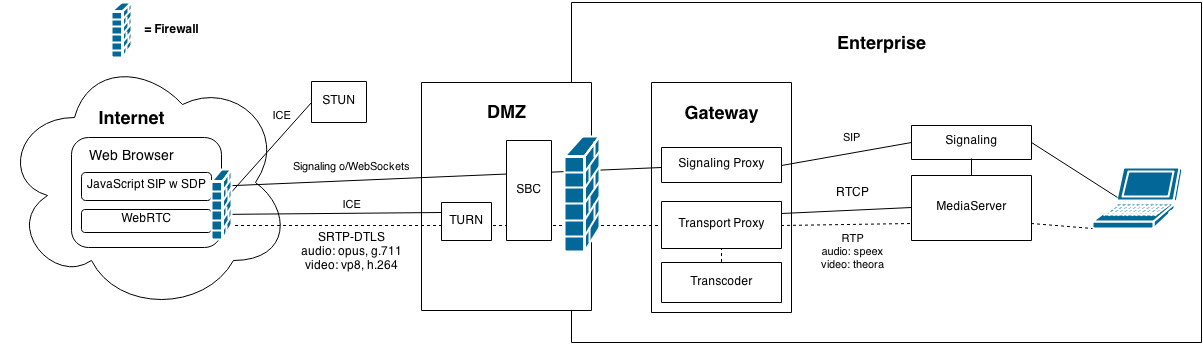
\includegraphics[scale=0.40]{gateway-final.png}}
\caption{WebRTC-Enterprise interworking architecture.}
\label{fig:gateway-final}
\end{figure}


\section{Evaluation}
My proposed solution turns out to be pretty similar in architecture to the 3GPP's TR 23.701\cite{3gpp-wrtc-access-ims} mentioned in section~\ref{sec:webrtc-ims}. The main difference is that TR 23.701 does not manage authentication of user identities, and it does not mention anything about media multiplexing. Although STUN is mentioned, there is no explicit mention of TURN support. Since implementing a working gateway was outside the scope of this thesis, I tested some of the components of the webrtc2sip gateway. I found that these worked quite well, and chose to use some of them in my model. I used SIP Proxy in the signaling proxy, and RTCWeb Breaker for the transport proxy. It's possible we could use the Media Coder as well, but I was not able to test it.